\section{Zapewnienie spójności danych}

\begin{frame}{Spójność danych}
	
	\begin{alertblock}{Spójność/integralność danych}
		Możliwość stwierdzenia, że dane nie zostały nieautoryzowanie zmienione, dodane, usunięte.
	\end{alertblock}

	\begin{itemize}
		\item Szalenie ważne jest, abyśmy mogli stwierdzić z \emph{dużą dozą pewności}, iż dane po stronie odbiorcy i nadawcy są dokładnie takie same.
		
		\item Chcielibyśmy móc to sprawdzić, przesyłając znacząco mniej danych niż same dane.
		
		\item Do tego celu fenomenalnie nadają się kryptograficzne funkcje hashujące.
		
	\end{itemize}	

\end{frame}

\begin{frame}{Kryptograficzne funkcje haszujące}
	
	\begin{alertblock}{Kryptograficzna funkcja haszująca}
		Funkcja haszująca (f. skrótu) bezpieczna do zastosowań kryptograficzych; dla stosunkowo dużych danych wejściowych zwraca stosunkowo małą liczbę, typowo 128--512 bitów.
	\end{alertblock}
	
	Własności:\begin{itemize}
		\item najdrobniejsza zmiana danych wejściowych --- np. flipnięcie 1 bitu wśród 100 GiB --- całkowicie zmienia wyjście tej funkcji,
		\item danej wartości funkcji jest niesłychanie trudno spreparować generujące ją wejście,
		\item jeśli odbiorca i nadawca porównają kryptograficzny skrót ze swych kopii danych, i jeśli skróty te będą takie same, z dość \emph{dużym prawdopodobieństwem} dane są identyczne.
	\end{itemize}
	
\end{frame}

\begin{frame}{Prawdopodobieństwo kolizji dla 128-bitowej funkcji}
	
	W poprzednim slajdzie mówimy o \emph{dużym prawdopodobieństwie}:

	\begin{itemize}
		\item Prawdopodobieństwo kolizji dla dwóch hashy przy 128-bitowej zwracanej liczbie to $\frac{1}{2^{128}}=\frac{1}{340282366920938463463374607431768211456}$.
		
		\item Jeśli jednak weźmiemy pod uwagę \href{http://en.wikipedia.org/wiki/Birthday_problem}{paradoks urodzin}, możemy uzyskać prawdopodobieństwo kolizji $\frac{1}{2}$ wśród $2^{64}$ takich haszy.
		
		\item ... czyli np. haszując 6 \emph{miliardów} plików na sekundę przez następne 100 lat, hasze którychś dwu będą kolidować ze sobą prawdopodobieństwem $\frac{1}{2}$. :-)
	\end{itemize}	
	
\end{frame}

\begin{frame}{MD5}
	\begin{itemize}
		\item Wynaleziona w 1991 przez Rona Rivesta z MIT.
		\item Popularna kryptograficzna funkcja haszująca.
		\item Zwraca 128-bitową liczbę.
		\item W 2004 znaleziono sposób na generowanie kolizji...
		\item ... dlatego odradza się używanie jej.
	\end{itemize}
\end{frame}

\begin{frame}{SHA-1}
	\begin{itemize}
		\item Opublikowana w 1995 przez NSA.
		\item Popularna kryptograficzna funkcja haszująca.
		\item Zwraca 160-bitową liczbę.
		\item W 2005--2008 opublikowano m.in. atak, który wymaga $2^{63}$ operacji funkcji kompresującej, żeby znaleźć kolizję (w porównaniu do $2^{80}$ przy brute-force)...
		\item ... dlatego SHA-1 nie powinna być używana w nowych aplikacjach.
	\end{itemize}
\end{frame}

\begin{frame}{SHA-2}
	\begin{itemize}
		\item 4 funkcje zaprojektowane w 2001 przez NSA.
		\item Bitowości: SHA-224, SHA-256 oraz SHA-384, SHA-512.
		\item Do tej pory nie znaleziono kolizji.
	\end{itemize}
\end{frame}

\begin{frame}{Podpis cyfrowy}
	\begin{alertblock}{Podpis cyfrowy}
		Schemat pozwalający na zweryfikowanie, czy wiadomość została stworzona przez wiarygodnego nadawcę. Gwarantuje, że jej treść nie była modyfikowana podczas transmisji danych.
	\end{alertblock}	
	Algorytmy wykorzystujące podpis cyfrowy są powrzechnie wykorzystywane	 do uwierzytelniania i zapewniania spójności danych podczas transakcji finansowych oraz dystrybucji oprogramowania. 
\end{frame}

\begin{frame}{Podpis cyfrowy}
		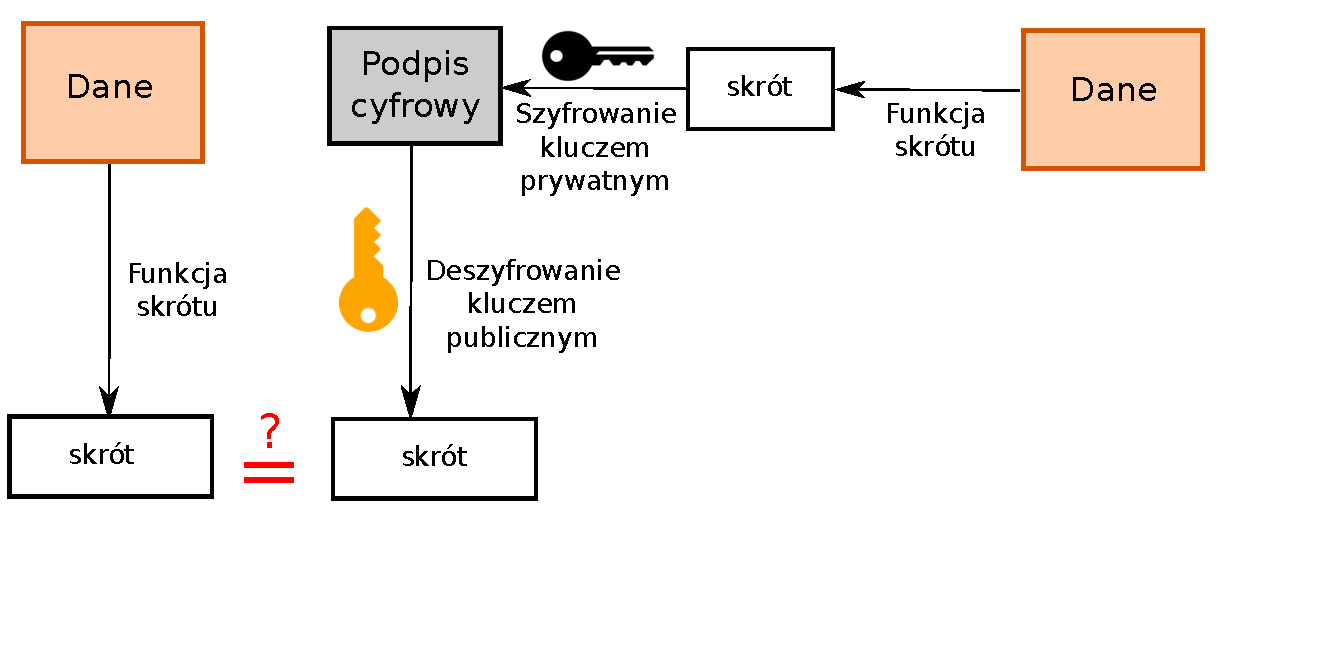
\includegraphics[height=0.5\paperwidth]{images/dig-sign.pdf}
\end{frame}
